% --------------------------------------------------------------
% This is all preamble stuff that you don't have to worry about.
% Head down to where it says "Start here"
% --------------------------------------------------------------
 
\documentclass[12pt]{article}
 
\usepackage[margin=1in]{geometry} 
\usepackage{amsmath,amsthm,amssymb}
 
\newcommand{\N}{\mathbb{N}}
\newcommand{\Z}{\mathbb{Z}}
 
\newenvironment{theorem}[2][Theorem]{\begin{trivlist}
\item[\hskip \labelsep {\bfseries #1}\hskip \labelsep {\bfseries #2.}]}{\end{trivlist}}

\newenvironment{lemma}[2][Lemma]{\begin{trivlist}
\item[\hskip \labelsep {\bfseries #1}\hskip \labelsep {\bfseries #2.}]}{\end{trivlist}}

\newenvironment{exercise}[2][Exercise]{\begin{trivlist}
\item[\hskip \labelsep {\bfseries #1}\hskip \labelsep {\bfseries #2.}]}{\end{trivlist}}

\newenvironment{problem}[2][Part]{\begin{trivlist}
\item[\hskip \labelsep {\bfseries #1}\hskip \labelsep {\bfseries #2}]}{\end{trivlist}}

\newenvironment{intro}[2][Introduction]{\begin{trivlist}
\item[\hskip \labelsep {\bfseries #1}\hskip \labelsep {\bfseries #2}]}{\end{trivlist}}

\newenvironment{question}[2][Question]{\begin{trivlist}
\item[\hskip \labelsep {\bfseries #1}\hskip \labelsep {\bfseries #2.}]}{\end{trivlist}}

\newenvironment{corollary}[2][Corollary]{\begin{trivlist}
\item[\hskip \labelsep {\bfseries #1}\hskip \labelsep {\bfseries #2.}]}{\end{trivlist}}

\usepackage{graphicx}
\graphicspath{{./}}

\newcommand{\bestBeta}{0.4}

\begin{document}
 
% --------------------------------------------------------------
%                         Start here
% --------------------------------------------------------------
 
\title{Project 2: Texture Modeling and Synthesis}%replace X with the appropriate number
\author{Yunzhong He\\ %replace with your name
204010749} %if necessary, replace with your course title
 
\maketitle

\begin{problem}{I Objective}
\item{}
This project uses minimax entropy principle to learn texture models from different images, and uses Gibbs sampling to synthesize images with similar patterns.
\begin{center}
	
\includegraphics[width=3cm]{Code/filter_1.png}
	
\includegraphics[width=3cm]{Code/filter_2.png}
	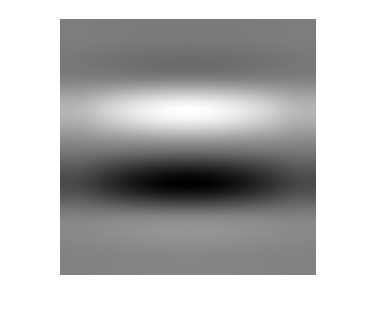
\includegraphics[width=3cm]{Code/filter_3.png}
	
\includegraphics[width=3cm]{Code/filter_4.png}
\end{center}
\end{problem}

\begin{problem}{II Filters}
\item{}
For this project we used 6 gradient filters of different directions, Gabor filters of sizes 7, 9, 15 and each with 6 different orientations, and 64 Dirac delta functions that only look at individual pixels in 8x8 windows. Below are some example filters.
\end{problem}

\begin{problem}{III Methods}
\item{III.1 Image pre-processing\\}
Before learning our model, we resized all images to 256x256 with 0~7 grayscale intensity to speed up our computations.
\item{III.2 Weighted histograms and filter selection\\}
Since it is more effective for histograms to match at head and tail, we assiged the weights \[8, 7, 6, 5, 4, 3, 2, 1, 2, 3, 4, 5, 6, 7, 8\] to our 15 bins. And we use the weights compute weighted difference between histograms. At each iteration, we pick the filter that yields the largest weighted histogram difference the input image and the synthesized result from the previous iteration. To pick an initial value for synthesized image, we simply generated a white noise image.
\end{problem}

\begin{problem}{IV Results}
\item{}
The following synthesized images and their corresponding L-1 error curves are achieved.
\item{IV.1 Fur}
\begin{center}
	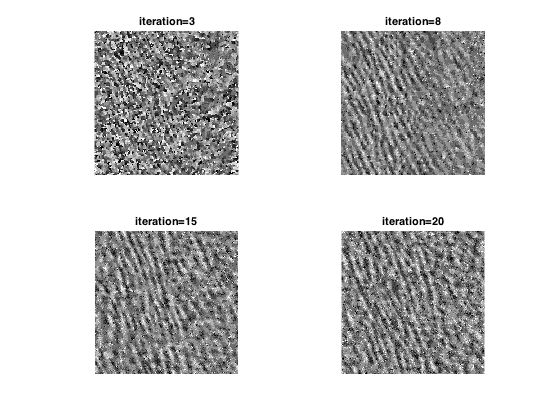
\includegraphics[width=14cm]{Code/Results/fur.png}
	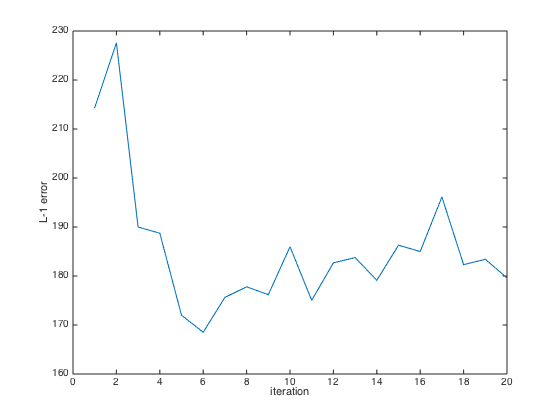
\includegraphics[width=10cm]{Code/Results/fur_error.png}
\end{center}
\item{IV.2 Grass}
\begin{center}
	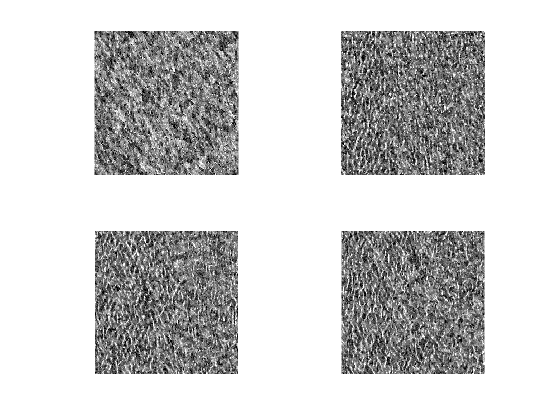
\includegraphics[width=14cm]{Code/Results/grass.png}
	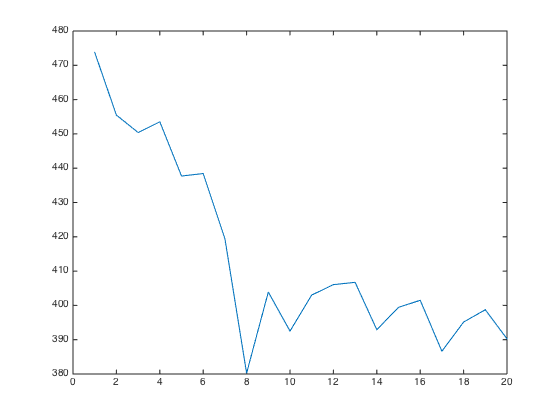
\includegraphics[width=10cm]{Code/Results/grass_error.png}
\end{center}
\item{Iv.3 Stucco}
\begin{center}
	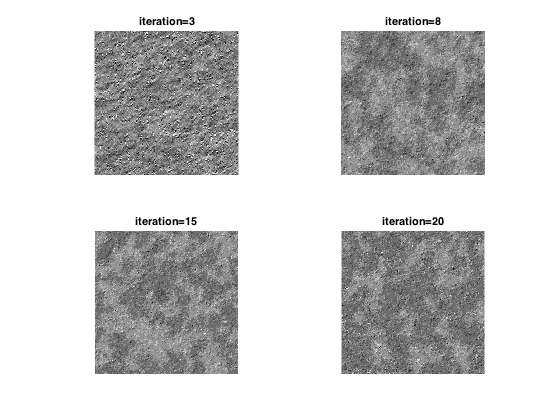
\includegraphics[width=14cm]{Code/Results/stucco.png}
	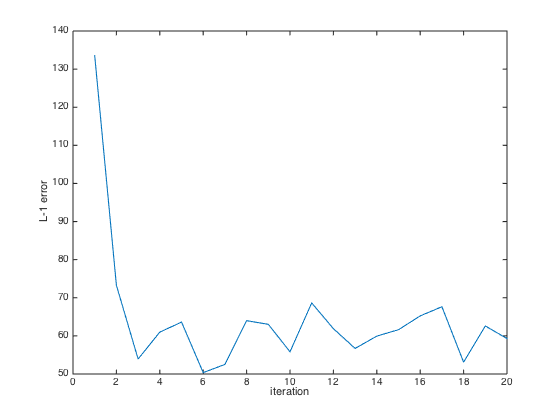
\includegraphics[width=10cm]{Code/Results/stucco_error.png}
\end{center}
\end{problem}
% --------------------------------------------------------------
% --------------------------------------------------------------
%     You don't have to mess with anything below this line.
% --------------------------------------------------------------
 
\end{document}
